\documentclass[10pt, a4paper, twocolumn]{article}

% ============================================================================
% PREAMBLE
% ============================================================================
\usepackage[utf8]{inputenc}
\usepackage{amsmath}
\usepackage{mathtools} % Added for split/multline
\usepackage{amssymb}
\usepackage{graphicx}
\usepackage{booktabs}
\usepackage{hyperref}
\usepackage{float}
\usepackage{listings}
\usepackage{xcolor}
\usepackage{geometry}
\usepackage{siunitx}
\usepackage{tikz}
\usetikzlibrary{shapes.geometric, arrows.meta, positioning, fit, backgrounds}
\geometry{margin=2cm}

% SI Units Configuration
\sisetup{
    per-mode=symbol,
    range-phrase=--,
    range-units=single,
    inter-unit-product=\ensuremath{{}\cdot{}}
}

% Code Listing Style (consolidated in preamble)
\lstset{
    language=Python,
    basicstyle=\footnotesize\ttfamily,
    keywordstyle=\color{blue},
    commentstyle=\color{gray},
    stringstyle=\color{orange},
    frame=single,
    breaklines=true,
    numbers=left,
    numberstyle=\tiny\color{gray},
    xleftmargin=2em,
    framexleftmargin=1.5em,
    aboveskip=1em,
    belowskip=1em
}

% ============================================================================
% DOCUMENT
% ============================================================================

\title{\textbf{Simulation Framework for Dual-Path Industrial Hydrogen Production v2.0: \\ Architecture, Physics, and High-Frequency Optimization}}
\author{Technical Engineering Team}
\date{December 2025}

\begin{document}

\maketitle

% ============================================================================
% ABSTRACT
% ============================================================================
\begin{abstract}
This paper presents the architectural and mathematical specification for the Dual-Path Hydrogen Production System v2.0. The framework provides a high-fidelity, event-driven simulation environment for modeling industrial-scale hydrogen plants combining Grid-powered Electrolysis (PEM/SOEC) and Natural Gas Autothermal Reforming (ATR).

Version 2.0 introduces component-level design with 50+ physics models across 20 categories, replacing the system-level abstraction of v1.0. Key innovations include: (1)~a six-layer modular architecture with strict lifecycle contracts, (2)~Look-Up Table (LUT) caching on 2000-point $(P, T)$ grids achieving 50--200$\times$ speedup, (3)~Numba JIT compilation for iterative solvers, and (4)~a Split-Layer Control Architecture decoupling economic dispatch from physical outcomes.

The physics models employ rigorous governing equations including the Shomate polynomial for thermodynamic properties, the Ergun equation for packed bed pressure drop, and Stokes-law-based separation efficiency for cyclonic separators. The framework completes annual simulations (525,600 timesteps at \SI{1}{\minute} resolution) in under \SI{5}{\minute} on standard hardware, enabling rapid techno-economic analysis for capacity planning and hydrogen market participation.
\end{abstract}

\vspace{0.5em}
\noindent\textbf{Keywords:} Hydrogen, Process Simulation, Techno-Economic Analysis, PEM Electrolysis, SOEC, Python, Numba, Look-Up Tables

% ============================================================================
% NOMENCLATURE
% ============================================================================
\section*{Nomenclature}

\begin{table}[H]
\centering
\begin{tabular}{@{}llr@{}}
\toprule
\textbf{Symbol} & \textbf{Description} & \textbf{Unit} \\
\midrule
\multicolumn{3}{l}{\textit{Flow State Variables}} \\
$\dot{m}$ & Mass flow rate & kg/h \\
$P$ & Pressure & Pa \\
$T$ & Temperature & K \\
$x_i$ & Mass fraction of species $i$ & -- \\
$y_i$ & Mole fraction of species $i$ & -- \\
$\mathbf{x}$ & Composition vector $\{x_{\text{H}_2}, x_{\text{O}_2}, \ldots\}$ & -- \\
\midrule
\multicolumn{3}{l}{\textit{Thermodynamic Properties}} \\
$H$ & Specific enthalpy & J/kg \\
$S$ & Specific entropy & J/(kg$\cdot$K) \\
$C_p$ & Isobaric heat capacity & J/(kg$\cdot$K) \\
$\rho$ & Density & kg/m$^3$ \\
$k$ & Ratio of specific heats ($C_p/C_v$) & -- \\
\midrule
\multicolumn{3}{l}{\textit{Physical Constants}} \\
$R$ & Universal gas constant & \SI{8.314}{\joule\per\mole\per\kelvin} \\
$R_{\text{H}_2}$ & Specific gas constant (H$_2$) & \SI{4124}{\joule\per\kilogram\per\kelvin} \\
$T_{ref}$ & Reference temperature & \SI{298.15}{\kelvin} \\
$P_{ref}$ & Reference pressure & \SI{101325}{\pascal} \\
\midrule
\multicolumn{3}{l}{\textit{Efficiency and Performance}} \\
$\eta$ & Efficiency (subscripted) & -- \\
$\eta_{is}$ & Isentropic efficiency & -- \\
$\eta_F$ & Faraday efficiency & -- \\
\midrule
\multicolumn{3}{l}{\textit{Simulation Parameters}} \\
$t$ & Simulation time & h \\
$\Delta t$ & Timestep & \SI{1}{\minute} ($1/60$~h) \\
$\mathbf{U}$ & Internal state vector & (varies) \\
$\mathbf{S}$ & Stream state vector & (defined below) \\
\midrule
\multicolumn{3}{l}{\textit{Electrochemical Variables}} \\
$j$ & Current density & A/m$^2$ \\
$j_0$ & Exchange current density & A/m$^2$ \\
$\alpha$ & Charge transfer coefficient & -- \\
$F$ & Faraday constant & \SI{96485}{C/mol} \\
$z$ & Electron transfer number & -- \\
\midrule
\multicolumn{3}{l}{\textit{Separation and Transport}} \\
$\varepsilon$ & Bed porosity (void fraction) & -- \\
$\mu$ & Dynamic viscosity & Pa$\cdot$s \\
$D_p$ & Particle diameter & m \\
$d_{50}$ & Cut-size diameter (cyclone) & m \\
$N_e$ & Number of effective turns & -- \\
$u_s$ & Superficial velocity & m/s \\
\bottomrule
\end{tabular}
\end{table}

% ============================================================================
% SECTION 1: INTRODUCTION
% ============================================================================
\section{Introduction}

\subsection{Problem Definition}

The global transition to a hydrogen-based energy economy demands sophisticated modeling tools capable of handling the intrinsic complexity of hybrid production pathways. Industrial hydrogen production increasingly combines multiple technologies:
\begin{itemize}
    \item \textbf{Green Hydrogen}: Water electrolysis powered by renewable electricity (PEM, SOEC)
    \item \textbf{Blue Hydrogen}: Autothermal reforming (ATR) with carbon capture
\end{itemize}

Each pathway exhibits distinct operational characteristics, capital costs, and carbon footprints, creating a multi-objective optimization landscape that plant operators must navigate in real-time.

\vspace{0.5em}
Annual techno-economic assessments require simulation of 8,760 operating hours---or 525,600 timesteps at \SI{1}{\minute} resolution---creating a formidable computational challenge. Each timestep demands:
\begin{enumerate}
    \item Thermodynamic property calculations for multi-component gas mixtures
    \item Phase equilibrium computations for separation equipment
    \item Control logic evaluation for power allocation and arbitrage
\end{enumerate}

Naively implemented, each CoolProp equation-of-state evaluation requires approximately \SI{0.1}{\milli\second} to \SI{1}{\milli\second}. Multiplied by 50+ components and 26 million annual property calls, simulation time would extend to days or weeks.

\subsection{What's New in Version 2.0}
\label{sec:whats-new}

Based on the detailed component system guide, v2.0 introduces the following upgrades:

\begin{itemize}
    \item \textbf{Component-Level Design}: Build plants using individual components (PEM stacks, heat exchangers, pumps) rather than system-level abstractions
    \item \textbf{20 Component Categories}: 50+ implementations organized by functional area (electrolysis, separation, compression, thermal, storage, water systems)
    \item \textbf{Environment Manager}: Time-series environmental data (wind power availability from \texttt{wind\_data.csv}, electricity prices from \texttt{EnergyPriceAverage2023-24.csv}) accessible to all components via registry lookup
    \item \textbf{System Assignment}: Context-dependent components (e.g., Rectifier, PSA Unit) can be assigned to specific systems (PEM/SOEC/ATR)
    \item \textbf{Backward Compatibility}: Both v1.0 (system-level) and v2.0 (component-level) configurations are supported
\end{itemize}

\subsection{Optimization Approach}

The system addresses the computational challenge through a multi-layered optimization approach:
\begin{enumerate}
    \item \textbf{Pre-computed Thermodynamic LUTs}: 2D interpolation grids on $(P, T)$ replace expensive CoolProp calls, achieving 50--200$\times$ speedup
    \item \textbf{Just-In-Time Compilation}: Numba-decorated numerical kernels compile to native machine code
    \item \textbf{Pre-allocated Memory}: NumPy arrays sized at initialization eliminate dynamic allocation
    \item \textbf{Causal Execution Ordering}: Component stepping follows mass and energy propagation paths
\end{enumerate}

% ============================================================================
% SECTION 2: SYSTEM ARCHITECTURE (METHODOLOGY)
% ============================================================================
\section{System Architecture}
\label{sec:architecture}

The software is constructed upon a six-layer modular architecture designed to ensure separation of concerns and scalability.

\subsection{Layered Design}

The architectural hierarchy progresses from foundational abstractions to user-facing interfaces:

\begin{table}[H]
\centering
\caption{Six-Layer Architecture Overview}
\label{tab:layers}
\begin{tabular}{@{}clp{3.5cm}@{}}
\toprule
\textbf{Layer} & \textbf{Purpose} & \textbf{Key Classes} \\
\midrule
1 & Core Foundation & \texttt{Component}, \texttt{Stream}, \texttt{ComponentRegistry} \\
2 & Performance & \texttt{LUTManager}, \texttt{numba\_ops} \\
3 & Components & 50+ physics models (20 categories) \\
4 & Orchestration & \texttt{PlantGraphBuilder}, \texttt{DualPathCoordinator} \\
5 & Simulation & \texttt{SimulationEngine}, \texttt{FlowNetwork} \\
6 & UI/Reporting & PySide6 editors, \texttt{markdown\_report} \\
\bottomrule
\end{tabular}
\end{table}

\vspace{1em}

\subsection{Component Lifecycle Contract}
\label{sec:lifecycle}

Every simulation entity inherits from the abstract \texttt{Component} base class, ensuring uniform behavior. The lifecycle contract formalizes three distinct phases:

\begin{lstlisting}[caption={Component Lifecycle Interface}]
class Component(ABC):
    @abstractmethod
    def initialize(self, dt: float, 
                   registry: ComponentRegistry):
        """Allocate memory, resolve dependencies."""
        
    @abstractmethod
    def step(self, t: float):
        """Advance state by one timestep."""
        
    @abstractmethod
    def get_state(self) -> Dict[str, Any]:
        """Return JSON-serializable state."""
\end{lstlisting}

\vspace{0.5em}
\textbf{Initialization Phase}: Called once before simulation. Components allocate internal data structures (NumPy arrays sized for simulation duration), resolve dependencies via \texttt{ComponentRegistry}, and validate configuration.

\textbf{Stepping Phase}: Called every timestep with simulation time $t$. Components process inputs via \texttt{receive\_input()}, execute physics models, and prepare outputs for downstream consumers.

\textbf{State Access Phase}: Components expose internal state through \texttt{get\_state()}, enabling checkpoint persistence and monitoring.

\subsection{Data Flow Patterns}

The architecture implements distinct patterns for physics data and control signals:

\subsubsection{Push Architecture (Stream Propagation)}

Mass and energy flow downstream via the \texttt{Stream} dataclass:
\begin{center}
\texttt{Producer.step()} $\rightarrow$ \texttt{Downstream.receive\_input(stream)}
\end{center}

Each producer calculates outputs and pushes them to connected consumers. The \texttt{FlowNetwork} orchestrates this propagation after all components have stepped.

\subsubsection{Pull Architecture (Control Flow)}

Control and monitoring data flow upstream via registry queries:
\begin{center}
\texttt{Dispatch.record\_post\_step()} $\rightarrow$ \texttt{component.get\_state()}
\end{center}

The dispatch strategy queries actual component states after physics execution to record outcomes that may differ from commanded setpoints.

\begin{figure}[H]
\centering
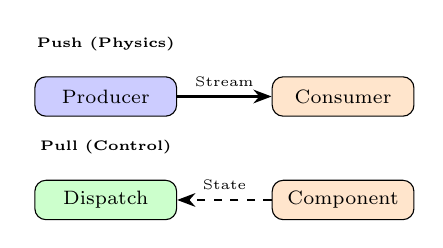
\begin{tikzpicture}[
    node distance=0.6cm,
    box/.style={rectangle, draw, rounded corners, minimum width=1.8cm, minimum height=0.5cm, font=\scriptsize},
    arrow/.style={-Stealth, thick}
]
    % Push flow
    \node[box, fill=blue!20] (prod) {Producer};
    \node[box, fill=orange!20, right=1.2cm of prod] (cons) {Consumer};
    \draw[arrow] (prod) -- node[above, font=\tiny] {Stream} (cons);
    \node[above=0.2cm of prod, font=\tiny\bfseries] {Push (Physics)};
    
    % Pull flow
    \node[box, fill=green!20, below=0.8cm of prod] (disp) {Dispatch};
    \node[box, fill=orange!20, right=1.2cm of disp] (comp) {Component};
    \draw[arrow, dashed] (comp) -- node[above, font=\tiny] {State} (disp);
    \node[above=0.2cm of disp, font=\tiny\bfseries] {Pull (Control)};
\end{tikzpicture}
\caption{Push vs. Pull Data Flow Patterns}
\label{fig:push-pull}
\end{figure}

\subsection{The Registry Pattern}

The \texttt{ComponentRegistry} serves as the central orchestrator for dependency injection:

\begin{equation}
    T_\text{lookup} = O(1) \quad \text{(hash-based dictionary access)}
\end{equation}

This pattern provides:
\begin{itemize}
    \item \textbf{Decoupled Dependencies}: Components depend on string IDs, not concrete class references
    \item \textbf{Lazy Resolution}: Dependencies resolved at initialization, avoiding circular imports
    \item \textbf{Type-Indexed Queries}: Retrieve components by category (e.g., ``storage'')
    \item \textbf{State Aggregation}: Single \texttt{get\_all\_states()} call for checkpointing
\end{itemize}

\subsection{Event-Driven Architecture}

The simulation combines continuous physics with discrete events via the \texttt{EventScheduler}:

\begin{equation}
    \text{Timestep} = \underbrace{\text{Events}}_{\text{Discrete}} + \underbrace{\text{Physics}}_{\text{Continuous}} + \underbrace{\text{Flows}}_{\text{Network}}
\end{equation}

Event types include maintenance scheduling, price updates, setpoint changes, and recurring actions (e.g., SOEC module priority rotation).

\subsection{Execution Flow \& Orchestration}
\label{sec:execution-flow}

The \texttt{SimulationEngine} does not merely iterate through timesteps; it orchestrates a strict multi-phase cycle that ensures consistency between \textbf{Economic Intent} (what the dispatch strategy commands) and \textbf{Physical Result} (what the thermodynamics permit).

\subsubsection{Anatomy of a Timestep: The 3-Phase Loop}

Each timestep $t$ follows a rigorous three-phase execution pattern:

\paragraph{Phase 1: Decision (Pre-Step)}
The dispatch system, implemented via the \texttt{HybridArbitrageEngineStrategy} (a concrete realization of the abstract \texttt{EngineDispatchStrategy}), analyzes current conditions---electricity spot prices, hydrogen selling prices, and wind power availability---to calculate optimal power allocation:

\begin{center}
\texttt{dispatch\_strategy.decide\_and\_apply(t, prices, wind)}
\end{center}

This phase produces \textit{setpoints} (Intent), which are injected into components via \texttt{receive\_input()}. For example, the dispatch may command the PEM electrolyzer to operate at \SI{2.5}{\mega\watt}, representing the economically optimal split between grid sales and hydrogen production.

\paragraph{Phase 2: Physics (Step)}
The \texttt{ComponentRegistry} orchestrates component execution in causal order:

\begin{center}
\texttt{for component in execution\_order:} \\
\hspace{2em}\texttt{component.step(t)}
\end{center}

The \textit{actual} physics happens here. Crucially, physical constraints may override economic commands. For example:
\begin{itemize}
    \item A \SI{2.5}{\mega\watt} setpoint may result in only \SI{2.1}{\mega\watt} actual consumption if the stack reaches thermal limits
    \item Compressor throughput may be curtailed if discharge temperature exceeds \SI{150}{\celsius}
    \item Storage tanks may refuse inflow if pressure exceeds $P_\text{max}$
\end{itemize}

After all components have stepped, the \texttt{FlowNetwork} propagates streams through the topology:

\begin{center}
\texttt{flow\_network.execute\_flows(t)}
\end{center}

This ``Push'' propagation delivers output streams from producers to connected consumers via \texttt{receive\_input()}.

\paragraph{Phase 3: Recording (Post-Step)}
The dispatch strategy queries \textit{actual} component states to record outcomes:

\begin{center}
\texttt{dispatch\_strategy.record\_post\_step()}
\end{center}

This phase reads operational metrics via \texttt{get\_state()} and writes them to pre-allocated NumPy arrays. The recorded values reflect what \textit{actually happened}, not what was \textit{commanded}---enabling accurate techno-economic analysis.

\subsubsection{Concrete Example: Wind to Hydrogen}

Consider wind power becoming available at timestep $t$:

\begin{enumerate}
    \item \textbf{Decision}: Dispatch calculates that producing hydrogen yields higher value than grid export. Commands \SI{5}{\mega\watt} to PEM electrolyzer via \texttt{pem.receive\_input('power\_setpoint', 5000, 'kW')}.
    
    \item \textbf{Physics}: PEM executes \texttt{step(t)}:
    \begin{itemize}
        \item Calculates $\dot{m}_{\text{H}_2}$ from Faraday's law
        \item Creates output \texttt{Stream(mass\_flow=45.2, T=353, P=3e6, composition=\{'H2': 0.98, 'H2O': 0.02\})}
    \end{itemize}
    
    \item \textbf{Flow Propagation}: \texttt{FlowNetwork} pushes the stream to the Knock-Out Drum:
    \begin{center}
    \texttt{kod.receive\_input('inlet', pem\_stream, 'gas')}
    \end{center}
    
    \item \textbf{Recording}: Dispatch reads \texttt{pem.get\_state()['actual\_power\_kw']} = 4850 (thermal de-rating) and stores in history array.
\end{enumerate}

\subsubsection{Algorithm: Main Simulation Loop}

Algorithm~\ref{alg:main-loop} formalizes the timestep execution using actual method names from the codebase.

\begin{figure}[H]
\begin{lstlisting}[caption={SimulationEngine Main Loop}, label=alg:main-loop, escapechar=|]
def run(start_hour, end_hour):
    # Initialization Phase
    registry.initialize_all(dt=dt_hours)
    flow_network.initialize()
    
    for step in range(start_step, end_step):
        hour = step / 60  # 1-minute resolution
        
        # --- Phase 1: Decision (Pre-Step) ---
        event_scheduler.process_events(hour, registry)
        if dispatch_strategy:
            dispatch_strategy.decide_and_apply(
                t=hour, prices=prices, wind=wind)
        
        # --- Phase 2: Physics (Step) ---
        for comp_id in execution_order:
            registry.get(comp_id).step(hour)
        
        flow_network.execute_flows(hour)
        
        # --- Phase 3: Recording (Post-Step) ---
        if dispatch_strategy:
            dispatch_strategy.record_post_step()
        
        monitoring.collect(hour, registry)
\end{lstlisting}
\end{figure}

\subsubsection{Causal Execution Order}

Component ordering ensures upstream calculations complete before downstream consumption. The default order follows mass/energy propagation:

\begin{enumerate}
    \item \textbf{External Inputs}: \texttt{environment\_manager}, \texttt{energy\_price\_tracker}
    \item \textbf{Coordination}: \texttt{dual\_path\_coordinator}
    \item \textbf{Production}: \texttt{soec\_cluster}, \texttt{pem\_electrolyzer}
    \item \textbf{Thermal}: \texttt{thermal\_manager}, \texttt{chiller}
    \item \textbf{Separation}: \texttt{knock\_out\_drum}, \texttt{psa}
    \item \textbf{Compression}: \texttt{compressor\_c1}, \texttt{compressor\_c2}
    \item \textbf{Storage}: \texttt{lp\_tanks}, \texttt{hp\_tanks}
\end{enumerate}

This ordering minimizes the need for iterative convergence within each timestep.

% ============================================================================
% SECTION 3: MATHEMATICAL MODELING (METHODOLOGY)
% ============================================================================
\section{Mathematical Modeling}
\label{sec:math}

This section formalizes the mathematical abstraction underlying the simulation framework, establishing notation and governing principles before presenting component-specific equations.

\subsection{Thermodynamic State Vector}

The fundamental data structure for inter-component communication is the \textbf{Stream}, which encapsulates the complete thermodynamic state of a material flow. We define the flow state vector:

\begin{equation}
    \mathbf{S} = \begin{bmatrix} \dot{m} \\ P \\ T \\ \mathbf{x} \end{bmatrix} \quad \text{where} \quad \mathbf{x} = \{x_{\text{H}_2}, x_{\text{O}_2}, x_{\text{H}_2\text{O}}, \ldots\}
    \label{eq:state-vector}
\end{equation}

The composition vector $\mathbf{x}$ contains mass fractions satisfying the constraint $\sum_i x_i = 1$. Each component acts as a \textbf{transfer function} transforming an input stream to an output stream:

\begin{equation}
    \mathbf{S}_{out} = f_c(\mathbf{S}_{in}, \mathbf{U}_c, t)
    \label{eq:transfer-function}
\end{equation}

where $\mathbf{U}_c$ represents the internal state of component $c$ (e.g., tank inventory, stack temperature) and $t$ is time. This functional abstraction enables modular composition: complex plants are constructed by chaining transfer functions.

\subsection{Time Discretization}

The simulation advances using a fixed discrete timestep approach. Component internal states evolve according to:

\begin{equation}
    \frac{d\mathbf{U}}{dt} = g(\mathbf{U}, \mathbf{S}_{in}, t)
    \label{eq:ode}
\end{equation}

This ODE is integrated using an explicit Euler scheme:

\begin{equation}
    \mathbf{U}^{n+1} = \mathbf{U}^n + \Delta t \cdot g(\mathbf{U}^n, \mathbf{S}_{in}^n, t^n)
    \label{eq:euler}
\end{equation}

where $\Delta t = \SI{60}{\second} = 1/60~\text{h}$ and $n$ denotes the timestep index. For annual simulations, $n \in \{0, 1, \ldots, 525599\}$.

\textbf{Dimensional Note:} All rate quantities (e.g., $\dot{m}$) are stored in engineering units (kg/h) but are internally normalized to consistent time bases during integration. The timestep $\Delta t$ is expressed in hours when computing state updates to ensure dimensional homogeneity with mass flow rates.

The explicit scheme is chosen for:
\begin{itemize}
    \item \textbf{Simplicity}: No matrix inversion required
    \item \textbf{Speed}: Each component evaluates $g(\cdot)$ once per timestep
    \item \textbf{Stability}: The \SI{60}{\second} timestep is well below the Courant-Friedrichs-Lewy (CFL) limit for the physical processes modeled
\end{itemize}

\subsection{Conservation Laws}
\label{sec:conservation}

All components in the simulation obey fundamental conservation principles applied to control volumes. These balance equations form the theoretical foundation upon which component-specific physics are built.

\subsubsection{Mass Balance}

The time-dependent mass balance for a generic control volume with multiple inlets and outlets:

\begin{equation}
    \frac{dM}{dt} = \sum_j \dot{m}_{in,j} - \sum_k \dot{m}_{out,k}
    \label{eq:mass-balance}
\end{equation}

where $M$ is the mass inventory (kg), and $\dot{m}$ are mass flow rates (kg/h).

\subsubsection{Species Balance}

For each chemical species $i$ (H$_2$, O$_2$, H$_2$O, etc.):

\begin{equation}
    \frac{d(M x_i)}{dt} = \sum_j \dot{m}_{in,j} x_{i,j} - \sum_k \dot{m}_{out,k} x_{i,k} + r_i V
    \label{eq:species-balance}
\end{equation}

where $x_i$ is the mass fraction of species $i$, $r_i$ is the volumetric reaction rate (kg/m$^3$/h), and $V$ is the control volume (m$^3$). For non-reactive components (mixers, pipes, separators), $r_i = 0$.

\subsubsection{Energy Balance}

The first law of thermodynamics for an open system:

\begin{equation}
    \frac{dU}{dt} = \sum_j \dot{m}_{in,j} H_{in,j} - \sum_k \dot{m}_{out,k} H_{out,k} + \dot{Q} - \dot{W}
    \label{eq:energy-balance}
\end{equation}

where $U$ is internal energy (J), $H$ is specific enthalpy (J/kg), $\dot{Q}$ is heat transfer rate (W), and $\dot{W}$ is shaft work rate (W).

\subsubsection{Quasi-Steady Approximation}

For \textbf{quasi-steady} components---such as pipes, mixers, heat exchangers, and separators---the accumulation terms are negligible:

\begin{equation}
    \frac{dM}{dt} \approx 0, \quad \frac{dU}{dt} \approx 0
\end{equation}

This reduces the differential equations to \textbf{algebraic} constraints, significantly simplifying the computational burden. Only \textbf{dynamic} components (storage tanks, thermal masses, electrolyzer stacks) retain time-dependent accumulation terms.

\subsection{Thermodynamic Property Framework}
\label{sec:property-framework}

The simulation employs a \textbf{Hybrid Equation of State (EOS)} approach, balancing computational efficiency with physical accuracy.

\subsubsection{Equation of State}

\paragraph{Low-Pressure Gas Streams}
For gas-phase streams at moderate pressures ($P < \SI{50}{\bar}$), the \textbf{Ideal Gas Law} is used:

\begin{equation}
    \rho = \frac{P M_{mix}}{R T}
    \label{eq:ideal-gas}
\end{equation}

where $M_{mix}$ is the mixture molecular weight (kg/mol) and $R = \SI{8.314}{\joule\per\mole\per\kelvin}$.

\paragraph{High-Pressure Pure Fluids}
For high-pressure applications (compression, storage at $P > \SI{100}{\bar}$), \textbf{Look-Up Tables (LUTs)} derived from CoolProp provide accurate real-gas properties including compressibility effects.

\paragraph{Liquid Water}
Liquid water density is treated as incompressible: $\rho_{H_2O} = \SI{1000}{\kilogram\per\meter\cubed}$.

\subsubsection{Caloric Properties}

Specific heat capacity and enthalpy are derived from the \textbf{Shomate polynomial} (NIST database), which captures temperature dependence:

\begin{equation}
    C_p(T) = A + B\tau + C\tau^2 + D\tau^3 + \frac{E}{\tau^2} \quad [\text{J/(mol}\cdot\text{K)}]
    \label{eq:shomate-caloric}
\end{equation}

where $\tau = T/1000$. Coefficients $A, B, C, D, E, F$ are species-specific (stored in \texttt{constants.py}). This formulation replaces the simplistic constant-$C_p$ assumption with rigorous NIST-based temperature dependence.

\subsubsection{Mixing Rules}

Mixture properties are calculated using linear combination rules (Dalton's Law approximation for ideal gas mixtures):

\paragraph{Molar Properties}
\begin{equation}
    H_{mix} = \sum_i y_i H_i(T), \quad S_{mix} = \sum_i y_i S_i(T, P) - R \sum_i y_i \ln(y_i)
    \label{eq:mixing-enthalpy}
\end{equation}

where $y_i$ is the mole fraction of species $i$.

\paragraph{Mass-Basis Properties}
\begin{equation}
    C_{p,mix} = \sum_i x_i C_{p,i}(T), \quad M_{mix} = \left( \sum_i \frac{x_i}{M_i} \right)^{-1}
    \label{eq:mixing-mass}
\end{equation}

\paragraph{Kay's Rule for Pseudo-Critical Properties}
When compressibility corrections are needed, pseudo-critical properties are estimated via Kay's mixing rule:

\begin{equation}
    T_{c,mix} = \sum_i y_i T_{c,i}, \quad P_{c,mix} = \sum_i y_i P_{c,i}
    \label{eq:kays-rule}
\end{equation}

This enables reduced property calculations for real-gas corrections in high-pressure applications.

\subsection{Governing Physics Summary}

Table~\ref{tab:physics-summary} summarizes the physical principles governing each component category, referencing both conservation laws and component-specific equations.

\begin{table}[H]
\centering
\caption{Component Physics Summary}
\label{tab:physics-summary}
\begin{tabular}{@{}lll@{}}
\toprule
\textbf{Component} & \textbf{Physical Principle} & \textbf{Equation} \\
\midrule
Generic (all) & Mass conservation & Eq.~\ref{eq:mass-balance} \\
Generic (all) & Energy conservation & Eq.~\ref{eq:energy-balance} \\
\midrule
Compressor & Isentropic work & Eq.~\ref{eq:compressor} \\
KnockOutDrum & Rachford-Rice VLE & Eq.~\ref{eq:rachford-rice} \\
TSA Unit & Ergun pressure drop & Eq.~\ref{eq:ergun} \\
Multi-Cyclone & Stokes settling & Eq.~\ref{eq:stokes} \\
PEM & Tafel kinetics & Eq.~\ref{eq:tafel} \\
SOEC & Operating curve & Table~\ref{tab:soec-states} \\
Storage Tank & Ideal gas accumulation & Eq.~\ref{eq:tank-dynamics} \\
\bottomrule
\end{tabular}
\end{table}

\vspace{1em}

\subsection{Component-Specific Physics}

The following subsections detail the physics models for specific component categories. All components inherit the conservation laws from Section~\ref{sec:conservation} and property calculations from Section~\ref{sec:property-framework}.

\subsubsection{Caloric Property Integration}

Enthalpy is computed by integrating the Shomate $C_p$ polynomial (Eq.~\ref{eq:shomate-caloric}) from reference temperature $T_{ref}$:

\begin{equation}
    H(T) - H(T_{ref}) = A\tau + \frac{B\tau^2}{2} + \frac{C\tau^3}{3} + \frac{D\tau^4}{4} - \frac{E}{\tau} + F
    \label{eq:enthalpy-integration}
\end{equation}

where $\tau = T/1000$. This is distinct from simulation time $t$.

\subsubsection{Compression Systems}
\label{sec:compression}

The framework distinguishes between two compression regimes based on pressure differential and thermal constraints.

\paragraph{Regime A: Adiabatic Single-Stage}
Implemented in \texttt{CompressorSingle}, this model applies to low-pressure differentials ($r_p < 4.0$), such as Balance-of-Plant (BoP) recirculation pumps or transfer compressors. The process is modeled as adiabatic compression corrected by isentropic efficiency $\eta_{is}$:

\begin{equation}
    W_{compressor} = \dot{m} \cdot \frac{H(P_{out}, S_{in}) - H(P_{in}, T_{in})}{\eta_{is}}
    \label{eq:compressor-adiabatic}
\end{equation}

The discharge temperature $T_{out}$ is obtained by solving the inverse enthalpy relation:
\begin{equation}
    T_{out} = T(P_{out}, H_{out}) \quad \text{where} \quad H_{out} = H_{in} + \frac{W_{compressor}}{\dot{m}}
\end{equation}

\paragraph{Regime B: Multi-Stage Intercooled}
Implemented in \texttt{CompressorStorage}, this model is used for high-pressure storage applications ($30 \to \SI{350}{\bar}$). The system minimizes work by approximating isothermal compression through $N$ stages of adiabatic compression followed by intercooling.

The number of stages $N$ is optimized to limit discharge temperature ($T_{out} \le T_{max}$):
\begin{equation}
    N = \left\lceil \frac{\ln(P_{target}/P_{suction})}{\ln(r_{max})} \right\rceil
\end{equation}

The stage pressure ratio $r_p$ assumes geometric progression:
\begin{equation}
    r_p = \left( \frac{P_{target}}{P_{suction}} \right)^{1/N}
\end{equation}

Total power is the summation of individual stage work, with fluid temperature reset to $T_{cool}$ (typically \SI{40}{\celsius}) between stages:
\begin{equation}
\begin{split}
    P_{total} = \dot{m} \sum_{i=1}^{N} \frac{1}{\eta_{is}} \Big[ H(P_{i,out}, S_{in,i}) \\
    - H(P_{i,in}, T_{in,i}) \Big]
\end{split}
\end{equation}

\textbf{Implementation Note:} Enthalpy changes $\Delta H$ and entropy $S$ are dynamically calculated using the Shomate polynomial or LUTs (Section~\ref{sec:property-framework}), capturing real-gas behavior where $C_p(T)$ and $Z(P,T)$ vary significantly.

\subsubsection{Electrolysis Systems}
\label{sec:electrolysis}

The plant employs two distinct electrolysis technologies, modeled with fidelities appropriate to their operational dynamics.

\paragraph{PEM Electrolysis (Polarization Model)}
The Proton Exchange Membrane (PEM) electrolyzer (`DetailedPEMElectrolyzer`) utilizes a mechanistic electrochemical model. The cell voltage $V_{cell}$ is calculated by summing the reversible potential and overpotential losses:

\begin{equation}
    V_{cell}(j, T, P) = V_{rev} + V_{act} + V_{ohm} + V_{conc}
\end{equation}

where $j$ is current density ($\text{A/cm}^2$). The reversible potential $V_{rev}$ follows the Nernst equation:

\begin{equation}
    V_{rev} = V^0 + \frac{RT}{2F} \ln\left( \frac{P_{H_2} P_{O_2}^{0.5}}{a_{H_2O}} \right)
\end{equation}

Hydrogen production rate is derived from Faraday's Law, accounting for efficiency losses ($\eta_F$) due to crossover:

\begin{equation}
    \dot{m}_{H_2} = N_{cells} \cdot \frac{I}{2F} \cdot M_{H_2} \cdot \eta_F(j)
\end{equation}

\paragraph{SOEC Electrolysis (Operational Model)}
The Solid Oxide Electrolyzer (`SOECOperator`) is modeled as a thermodynamic state machine due to the dominance of thermal transients in ceramic stacks. The system operates in discrete states $S \in \{\text{OFF}, \text{RAMP}, \text{STEADY}, \text{STANDBY}\}$.

Production is governed by specific energy consumption maps $E_{spec}(t_{age})$ derived from degradation curves, reflecting the thermodynamic advantage of steam splitting ($\sim 37.5$ kWh/kg):

\begin{equation}
    \dot{m}_{H_2} = \frac{P_{load}}{E_{spec}(t_{age})}
\end{equation}

Thermal gating logic prevents load changes until stack temperature stabilizes, capturing the high thermal inertia of the modules.

\subsubsection{Balance of Plant (Water Systems)}
\label{sec:water-systems}

Water circuit components (\texttt{WaterPump}, \texttt{PumpThermodynamic}) model incompressible flow dynamics. Unlike gas compressors, density $\rho$ is constant ($\approx \SI{1000}{\kilogram\per\cubic\meter}$):

\begin{equation}
    P_{pump} = \frac{\dot{m} \Delta P}{\rho \eta_{pump}}
    \label{eq:pump_power}
\end{equation}

Mass balance closure ensures continuous supply for electrolysis:
\begin{equation}
    \dot{m}_{water,in} = \sum \dot{m}_{cons, electrolyzers} + \dot{m}_{purge}
\end{equation}

\subsubsection{Thermal Management (Dry Coolers)}
\label{sec:thermal}

The indirect cooling system (\texttt{DryCooler}) rejects process heat $Q_{rej}$ to the ambient environment. The system operates under a rigid thermodynamic constraint: the outlet process temperature $T_{out}$ cannot drop below the ambient air temperature $T_{air}$ plus a minimum approach difference $\Delta T_{min}$:

\begin{equation}
    T_{out} \ge T_{air} + \Delta T_{min}
\end{equation}

Heat rejection is calculated using the $\varepsilon$-NTU method for cross-flow exchangers:

\begin{equation}
    Q_{rej} = \varepsilon \cdot C_{min} (T_{in} - T_{air})
\end{equation}

Unlike variable-load compressors, the air-cooler fan power is modeled as a fixed parasitic load $P_{fan}$ when active, derived from the nominal design air flow:

\begin{equation}
    P_{fan} = \frac{\dot{V}_{air} \Delta P_{air}}{\eta_{fan}}
\end{equation}

\subsubsection{Flow Control (Throttling Valves)}
\label{sec:valves}

Throttling valves (\texttt{ThrottlingValve}) are modeled as isenthalpic expansion devices (Joule-Thomson expansion). Assuming adiabatic operation and negligible kinetic energy changes:

\begin{equation}
    H(P_{in}, T_{in}) = H(P_{out}, T_{out})
    \label{eq:isenthalpic}
\end{equation}

While enthalpy $H$ is conserved, the outlet temperature $T_{out}$ is determined by querying the Equation of State (LUT or Shomate) to solve the inverse problem:

\begin{equation}
    T_{out} = T(P_{out}, H_{in})
\end{equation}

Crucially, for Hydrogen at standard conditions ($T > \SI{202}{\kelvin}$), the Joule-Thomson coefficient $\mu_{JT} < 0$. Consequently, expansion results in a temperature \textbf{increase}, contrasting with the cooling effect seen in standard gases.

\subsubsection{Mixing and Junction Systems}
\label{sec:mixing}

Unlike simplified simulators that employ linear temperature averaging ($T_{mix} \approx \sum w_i T_i$), this framework enforces **rigorous enthalpy and energy conservation**. This accounts for non-linear specific heat capacity $C_p(T)$ and phase behavior critical for detecting thermal anomalies.

\paragraph{Gas Phase Mixing}
The \texttt{MultiComponentMixer} operates in two thermodynamic modes depending on the physical context, utilizing **Newton-Raphson iteration** accelerated via **Numba JIT**:

\begin{itemize}
    \item \textbf{Continuous Mode (Pipe Junction)}: Solves a **PH-Flash** where specific enthalpy is conserved. The outlet temperature $T_{out}$ is found such that:
    \begin{equation}
        H_{mix}(P, T_{out}) = \frac{\sum \dot{m}_i H_i(T_i, P_i)}{\sum \dot{m}_i}
    \end{equation}

    \item \textbf{Batch Mode (Tank Filling)}: Solves a **UV-Flash** where internal energy is conserved within the rigid control volume. The internal energy accumulation equals the incoming enthalpy flow (flow work included):
    \begin{equation}
        U_{sys}(t+\Delta t) = U_{sys}(t) + \sum (\dot{m}_i H_i) \Delta t
    \end{equation}
\end{itemize}

\paragraph{Liquid Phase Mixing}
The \texttt{WaterMixer} implements **Adiabatic Isobaric Mixing**, essential for tracking thermal buildup in recirculation loops where $C_p$ varies with temperature:

\begin{enumerate}
    \item \textbf{Mass Balance}: $\dot{m}_{out} = \sum \dot{m}_i$
    \item \textbf{Enthalpy Balance}: $H_{out} = (\sum \dot{m}_i H_i) / \dot{m}_{out}$
    \item \textbf{State Resolution}: Invert Equation of State ($T_{out} = T(P_{out}, H_{out})$)
\end{enumerate}

\paragraph{Buffer Dynamics}
The \texttt{OxygenMixer} accounts for the thermal mass of gas buffers, applying First-Order Lag damping to temperature updates:

\begin{equation}
    T^{n+1} = \left(1 - \frac{\Delta t}{\tau}\right) T^n + \frac{\Delta t}{\tau} T_{target}
\end{equation}

Pressure is rigorously derived from density $\rho = M/V$ and temperature using the Real-Gas EOS:
\begin{equation}
    P = P_{EOS}(\rho, T)
\end{equation}

\subsubsection{Chemical Reaction Systems}
\label{sec:reactors}

This framework employs divergent modeling strategies for chemical reactors, selecting between mechanistic and surrogate approaches based on the balance between safety-critical dynamics and computational tractability.

\paragraph{Catalytic Purification (Deoxo PFR) [Mechanistic Model]}
The \texttt{DeoxoReactor} removes trace oxygen via the highly exothermic reaction $2H_2 + O_2 \to 2H_2O$ ($\Delta H_{rxn} = \SI{-242}{\kilo\joule\per\mole}$). Due to the safety risk of thermal runaway, a rigorous **Plug Flow Reactor (PFR)** model calculates spatial profiles ($dT/dL$, $dX/dL$) to detect hotspots.

The system solves coupled Ordinary Differential Equations (ODEs) using **Runge-Kutta 4th Order (RK4)** integration:

\begin{equation}
    \frac{dX_{O2}}{dL} = \frac{k(T) C_{O2} A_c}{\dot{F}_{O2,0}}
\end{equation}

\begin{equation}
    \frac{dT}{dL} = \frac{(-\Delta H_{rxn}) \dot{F}_{O2,0} \frac{dX}{dL} - U \pi D (T - T_{cool})}{\sum \dot{F}_i C_{p,i}}
\end{equation}

where $k(T)$ follows Arrhenius kinetics. This granularity ensures that catalyst temperature limits ($T < T_{max}$) are strictly enforced during transient startup.

\paragraph{Autothermal Reforming (ATR) [Surrogate Model]}
Simulating the complex kinetics of Autothermal Reforming (Partial Oxidation + Steam Reforming + Water-Gas Shift) is computationally prohibitive for real-time plant control. The \texttt{ATRReactor} therefore utilizes a **Data-Driven Surrogate Model**.

Yield curves derived from high-fidelity offline simulations (Aspen Plus) are mapped using **Numba-accelerated interpolation**:

\begin{equation}
    \mathbf{Y}_{out} = \mathcal{F}_{interp}(\dot{F}_{O2}, \dot{F}_{feed})
\end{equation}

This model captures the net effect of three simultaneous reactions:
\begin{itemize}
    \item \textbf{Partial Oxidation}: $CH_4 + 0.5O_2 \to CO + 2H_2$ ($\Delta H < 0$)
    \item \textbf{Steam Reforming}: $CH_4 + H_2O \rightleftharpoons CO + 3H_2$ ($\Delta H > 0$)
    \item \textbf{Water-Gas Shift}: $CO + H_2O \rightleftharpoons CO_2 + H_2$ ($\Delta H < 0$)
\end{itemize}

This approach ensures accurate mass/energy balances ($\pm 1\%$) while reducing calculation time by orders of magnitude compared to mechanistic CFD or Gibbs minimization solvers.

\subsubsection{Separation \& Purification}
\label{sec:separation}





\paragraph{Inertial Separation (Multi-Cyclone)}
The \texttt{HydrogenMultiCyclone} employs the **Barth/Muschelknautz Model** to determine the critical cut-size magnitude. Separation occurs when the centrifugal settling velocity exceeds the radial gas drift in the swirl tubes:

\begin{equation}
    v_{settling}(d_p) \ge v_{radial}
\end{equation}

The model solves for the particle diameter $d_{50}$ (50\% efficiency) using **Numba-accelerated iterations** to resolve the coupling between the tangential velocity field and particle drag coefficients. Pressure drop is derived from the geometric **Euler Number** ($\xi$) correlation:

\begin{equation}
    \Delta P = \xi \frac{\rho_g v_{axial}^2}{2}
\end{equation}

\paragraph{Aerosol Coalescence (Porous Media)}
For fine mist polishing ($d_p < \SI{0.1}{\micro\meter}$) where cyclones are ineffective, the \texttt{Coalescer} uses fibrous cartridge elements. Pressure drop is modeled via the **Carman-Kozeny Equation** for flow through porous media:

\begin{equation}
    \Delta P = K_{perm} \mu L_{elem} U_{sup}
\end{equation}

where $\mu$ follows the Sutherland power law ($\mu \propto T^{0.7}$). Unlike inertial separators, this component strictly accounts for **Dissolved Gas Losses** in the condensate. The mass of H$_2$/O$_2$ lost is calculated using Henry's Law constants ($H(T)$):

\begin{equation}
    \dot{m}_{gas,loss} = \dot{m}_{liq,rem} \cdot \frac{P_{partial}}{H(T)}
\end{equation}

This ensures rigorous mass conservation even for waste streams.

\paragraph{Gravity Separation (Knock-Out Drum)}
The \texttt{KnockOutDrum} removes bulk liquid via gravitational settling. To prevent liquid re-entrainment, the superficial gas velocity ($u_G$) must not exceed the terminal settling velocity derived from the **Souders-Brown Equation**:

\begin{equation}
    u_{max} = K_{SB} \sqrt{\frac{\rho_L - \rho_G}{\rho_G}}
    \label{eq:souders-brown}
\end{equation}

The component verifies that the vessel Diameter ($D$) is sufficient such that $u_{real} < u_{max}$. Separation equilibrium works as an **Isoenthalpic Flash**, solving the Rachford-Rice equation to determine the exact vapor-liquid split at inlet conditions.

\textit{Design Constraint}: For high-temperature process streams (e.g., SOEC anode exhaust at \SI{800}{\celsius}), active cooling (via \texttt{DryCooler}) is mandated \textbf{upstream} of the KOD. Direct connection of superheated vapor streams yields zero separation efficiency and violates the component's operational envelope.

\paragraph{Pressure Swing Adsorption (PSA)}
The \texttt{PSA} unit provides final purification (99.999\% purity) by removing trace impurities ($H_2O, N_2, CO_x$). Fluid dynamics through the packed adsorbent bed are modeled using the **Ergun Equation**:

\begin{equation}
    \frac{\Delta P}{L} = \frac{150 \mu u_s (1-\varepsilon)^2}{D_p^2 \varepsilon^3} + \frac{1.75 \rho_g u_s^2 (1-\varepsilon)}{D_p \varepsilon^3}
\end{equation}

where $\varepsilon$ is porosity and $D_p$ is particle diameter. Mass balance is governed by a fixed **Recovery Rate** ($R$), with the unrecovered hydrogen and all impurities rejected to the \texttt{tail\_gas} stream:

\begin{equation}
    \dot{m}_{tail} = \dot{m}_{in} - \dot{m}_{product}
\end{equation}

The unit operates in discrete cycles (Adsorption $\leftrightarrow$ Regeneration) defined by $t_{cycle}$, integrating power consumption for purge/vacuum operations.

\paragraph{Thermal Swing Adsorption (TSA)}
For temperature-driven purification, the \texttt{TSAUnit} uses dual packed beds where one absorbs moisture while the other regenerates. Pressure drop follows the same packed-bed mechanics as PSA (Eq. \ref{eq:ergun}). The primary constraint is the **Regeneration Energy Balance**:

\begin{equation}
    Q_{total} = \underbrace{m_{bed} C_{p,bed} \Delta T}_{Sensible} + \underbrace{m_{H_2O} \Delta H_{ads}}_{Desorption} + \underbrace{\dot{m}_{purge} C_{p,gas} \Delta T t_{cycle}}_{Purge~Heat}
\end{equation}

Heated purge gas (typically $\SI{250}{\celsius}$) drives the endothermic desorption process, regenerating the bed capacity for the next cycle.

\subsubsection{Storage Systems}
\label{sec:storage}

The storage module allows selecting between computational speed and physical fidelity depending on the simulation timescale.

\paragraph{Vectorized Tank Arrays (Low-Fidelity)}
Designed for grid-scale capacity planning, the \texttt{TankArray} implementation is a **Zero-Dimensional Mass Balance** model optimized for high-performance computing (HPC). It utilizes **Contiguous Memory Arrays** (NumPy) and **SIMD operations** (via Numba) to update thousands of tank states in a single CPU cycle.

Tanks transition between discrete states ($\mathcal{S} \in \{\text{CHARGING}, \text{DISCHARGING}, \text{IDLE}\}$) based on threshold logic. The global state update is vectorized:

\begin{equation}
    \mathbf{P}_{t+1} = \frac{\mathbf{m}_{t+1} R T}{\mathbf{V}} \quad (\text{ideal gas approximation})
\end{equation}

\paragraph{Dynamic Pressure Vessels (High-Fidelity)}
For compressor control loops and transient analysis, the \texttt{H2StorageTankEnhanced} acts as a **Dynamic Accumulator**. It solves the pressure derivative based on the Equation of State (EOS):

\begin{equation}
    \frac{dP}{dt} = \frac{(\dot{m}_{in} - \dot{m}_{out}) R Z T}{V}
\end{equation}

This model captures transient pressure spikes during filling and rapid depressurization effects, essential for validating safety relief valve (PRV) logic.

\subsubsection{Thermal Management \& Heat Recovery}
\label{sec:thermal_mgmt}

This section details the active heating/cooling units and passive recovery systems, distinguishing between parasitic loads (Boiler/Chiller) and efficiency enablers (Interchanger).

\paragraph{Active Heating (Electric Boiler)}
The \texttt{ElectricBoiler} functions as an **Isobaric Enthalpy Addition** device. Unlike simple temperature integrators, it determines the outlet state based on first-law efficiency ($\eta_{th}$):

\begin{equation}
    h_{out} = h_{in} + \frac{P_{elec} \eta_{th}}{\dot{m}}
\end{equation}

By solving the system in the enthalpy domain, the model automatically handles **Phase Transition** (Subcooled Liquid $\rightarrow$ Two-Phase $\rightarrow$ Superheated Steam). The outlet temperature is retrieved via the Equation of State inversion:

\begin{equation}
    T_{out} = \text{EOS}^{-1}(P, h_{out})
\end{equation}

This eliminates the need for complex "if-then" logic to track latent heat zones.

\paragraph{Active Cooling (Chiller)}
The \texttt{Chiller} calculates cooling load based on a dual-mode physics core to support both real fluids (steam/water) and ideal gases (hydrogen/oxygen):

\begin{equation}
    Q_{load} =
    \begin{cases}
    \dot{m}(h_{in} - h_{target}) & \text{Real Fluids (Captures Latent Heat)} \\
    \dot{m} C_p (T_{in} - T_{target}) & \text{Ideal Gas Fallback}
    \end{cases}
\end{equation}

Electrical consumption is derived from the **Coefficient of Performance (COP)**, representing the thermodynamic cost of heat rejection:

\begin{equation}
    P_{elec} = \frac{|Q_{load}|}{COP}
\end{equation}

\paragraph{Passive Recovery (Interchanger)}
The \texttt{Interchanger} is a counter-flow heat exchanger constrained by the **Second Law of Thermodynamics**. The actual heat transfer ($Q_{trans}$) is limited by the **Minimum Approach Temperature** ($\Delta T_{min}$) at the pinch point:

\begin{equation}
    Q_{trans} = \min(Q_{avail}, Q_{demand})
\end{equation}

where:

\begin{itemize}
    \item $Q_{avail} = \dot{m}_h C_{p,h} (T_{h,in} - (T_{c,in} + \Delta T_{min}))$
    \item $Q_{demand} = \dot{m}_c C_{p,c} (T_{target} - T_{c,in})$
\end{itemize}

This ensures physical realism by preventing temperature crossovers, modeling the finite surface area of real recuperators.

\paragraph{Centralized Heat Management (Virtual Heat Bus)}
The \texttt{ThermalManager} acts as a plant-wide supervisor, abstracting individual heat streams into a unified energy pool. It maximizes thermal efficiency ($\eta_{recovery}$) by continuously matching aggregate supply with process demand:

\begin{equation}
    Q_{utilized} = \min \left( \sum_{i} Q_{exhaust, i}, \sum_{j} Q_{sink, j} \right)
\end{equation}

where sources $Q_{exhaust}$ include electrolyzer stack cooling and compressor intercoolers, and sinks $Q_{sink}$ include feedwater pre-heating and SOEC steam generation. This virtualization decouples heat production from consumption, allowing for flexible "many-to-many" thermal integration without complex piping topology in the graph.

\subsubsection{Water Management \& Balance of Plant (BoP)}
\label{sec:water_mgmt_bop}

This section details the hydraulic control logic and thermodynamic consequences of the water recirculation loops.

\paragraph{Thermodynamic Pumping}
The \texttt{WaterPump} component extends standard hydraulic models by explicitly calculating the **Parasitic Heat Load** introduced by pump inefficiency. While the shaft power $P_{shaft}$ is defined by head requirements:

\begin{equation}
    P_{shaft} = \frac{\dot{m} v \Delta P}{\eta_{is} \eta_{mech}}
\end{equation}

The thermodynamic model captures the enthalpy rise in the fluid due to viscous dissipation ($1 - \eta_{is}$). For liquid water, this results in a temperature rise $\Delta T$ that accumulates in closed loops:

\begin{equation}
    \Delta T = \frac{\Delta H_{real}}{C_p} = \frac{v \Delta P}{\eta_{is} C_p}
\end{equation}

This effect, often neglected in simple flowsheets, significantly impacts the cooling load on downstream heat exchangers.

\paragraph{Inventory Control (Makeup Mixer)}
The \texttt{MakeupMixer} functions as an **Active Control Node** rather than a passive junction. It enforces a "Demand-Driven Injection" interaction to maintain constant loop inventory:

\begin{equation}
    \dot{m}_{makeup} = \max(0, \dot{m}_{target} - \dot{m}_{recycled})
\end{equation}

Thermodynamically, it solves the adiabatic mixing of cold makeup water ($T_{makeup}$) with the potentially hot recycled drain stream ($T_{recycled}$):

\begin{equation}
    T_{out} = \frac{\dot{m}_{recycled} T_{recycled} + \dot{m}_{makeup} T_{makeup}}{\dot{m}_{target}}
\end{equation}

The injection of cold makeup water acts as a stabilizing thermal sink, counteracting pump heat addition.

\paragraph{Closed-Loop Mass Accounting}
To validate the plant's environmental performance, the \texttt{WaterBalanceTracker} and \texttt{DrainRecorder} components implement rigorous mass conservation tracking. The \texttt{DrainRecorder} provides **Source Attribution**, distinguishing between liquid carryover from KODs versus aerosol capture in Coalescers.

System efficiency is quantified via the **Water Recovery Ratio (WRR)**:

\begin{equation}
    WRR = \frac{\sum \dot{m}_{recovered}}{\sum \dot{m}_{consumed}}
\end{equation}

This telemetry prevents "phantom mass generation" in the simulation and verifies that the closed-loop mass balance holds true over transient operation.

% ============================================================================
% SECTION 4: COMPUTATIONAL OPTIMIZATION (IMPLEMENTATION)
% ============================================================================
\section{Computational Optimization}
\label{sec:optimization}

\subsection{Look-Up Table Architecture}

The \texttt{LUTManager} implements a ``Generate Once, Cache Forever'' strategy for thermodynamic properties.

\subsubsection{Grid Specification}

Based on the architecture documentation:

\begin{table}[H]
\centering
\caption{LUT Grid Specification}
\label{tab:lut-spec}
\begin{tabular}{@{}lll@{}}
\toprule
\textbf{Axis} & \textbf{Range} & \textbf{Points} \\
\midrule
Pressure & \SI{0.05}{\bar} -- \SI{1000}{\bar} & 2000 (log spacing) \\
Temperature & \SI{273}{\kelvin} -- \SI{1200}{\kelvin} & 2000 (linear) \\
\bottomrule
\end{tabular}
\end{table}

\vspace{0.5em}
The grid uses 2D $(P, T)$ indexing with bilinear interpolation. The pressure axis uses geometric spacing (\texttt{np.geomspace}) to maintain resolution across four orders of magnitude.

\textbf{Properties cached}: Density ($D$), Enthalpy ($H$), Entropy ($S$), Heat Capacity ($C_p$), Compressibility ($Z$).

\textbf{Fluids}: H$_2$, O$_2$, H$_2$O, CO$_2$, CH$_4$, N$_2$.

\subsubsection{Cache Hit/Miss Mechanism}

\begin{itemize}
    \item \textbf{Cache Hit}: Query within bounds uses bilinear interpolation (\SI{0.5}{\micro\second} -- \SI{2}{\micro\second})
    \item \textbf{Cache Miss}: Out-of-bounds falls back to CoolProp (\SI{100}{\micro\second} -- \SI{1000}{\micro\second}), with logged warning
\end{itemize}

\subsection{JIT-Compiled Numerical Kernels}

The \texttt{numba\_ops} module provides Numba-decorated functions for hot paths:

\begin{lstlisting}[caption={JIT Flash Calculation}]
@njit
def solve_rachford_rice_single_condensable(
    z_condensable: float,
    K_value: float
) -> float:
    if K_value >= 1.0:  # Superheated
        return 1.0
    if z_condensable <= K_value:  # Undersaturated
        return 1.0
    # Two-phase solution
    beta = (1.0 - z_condensable) / (1.0 - K_value)
    return np.clip(beta, 0.0, 1.0)
\end{lstlisting}

% ============================================================================
% SECTION 5: INTEGRATED CONTROL ARCHITECTURE
% ============================================================================
\section{Integrated Control Architecture}

The system implements a Split-Layer Control Architecture separating economic intent from physical outcomes.

\subsection{Architecture Diagram}

\begin{figure}[H]
\centering
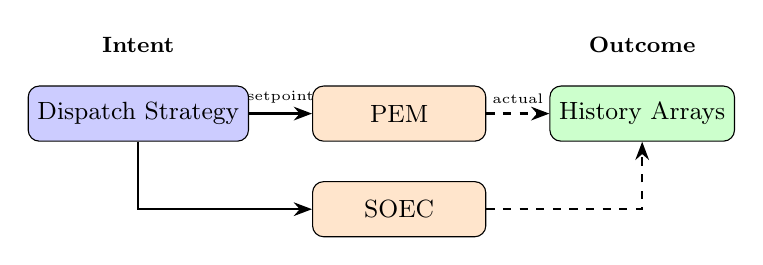
\begin{tikzpicture}[
    node distance=0.8cm,
    box/.style={rectangle, draw, rounded corners, minimum width=2.2cm, minimum height=0.7cm, font=\small},
    arrow/.style={-Stealth, thick}
]
    % Nodes
    \node[box, fill=blue!20] (dispatch) {Dispatch Strategy};
    \node[box, fill=orange!20, right=of dispatch] (pem) {PEM};
    \node[box, fill=orange!20, below=0.5cm of pem] (soec) {SOEC};
    \node[box, fill=green!20, right=of pem] (history) {History Arrays};
    
    % Arrows
    \draw[arrow] (dispatch) -- node[above, font=\tiny] {setpoint} (pem);
    \draw[arrow] (dispatch) |- (soec);
    \draw[arrow, dashed] (pem) -- node[above, font=\tiny] {actual} (history);
    \draw[arrow, dashed] (soec) -| (history);
    
    % Labels
    \node[above=0.3cm of dispatch, font=\footnotesize\bfseries] {Intent};
    \node[above=0.3cm of history, font=\footnotesize\bfseries] {Outcome};
\end{tikzpicture}
\caption{Split-Layer Control: Intent vs. Outcome}
\label{fig:control-arch}
\end{figure}

\subsection{Arbitrage Decision Logic}

The dispatch strategy compares selling electricity vs. producing hydrogen:

\begin{equation}
    P_\text{threshold} = P_\text{PPA} + \frac{1000}{\eta_\text{ref}} \times P_{\text{H}_2}
\end{equation}

When $P_\text{spot} > P_\text{threshold}$, selling power yields higher profit than hydrogen production.

% ============================================================================
% SECTION 6: ASSUMPTIONS AND VALIDITY
% ============================================================================
\section{Assumptions and Validity Range}
\label{sec:assumptions}

\subsection{Thermodynamic Assumptions}

\begin{itemize}
    \item \textbf{Ideal Gas Mixing}: Gas mixtures follow Kay's rule for pseudo-critical properties
    \item \textbf{Shomate Validity}: Equation~\ref{eq:shomate} is valid for \SI{273}{\kelvin} -- \SI{1500}{\kelvin}
    \item \textbf{Isothermal Storage}: Tanks assume constant temperature (no compression heating)
    \item \textbf{Single-Condensable VLE}: Flash calculations assume only H$_2$O condenses in H$_2$/O$_2$ carriers
\end{itemize}

\subsection{Numerical Assumptions}

\begin{itemize}
    \item \textbf{LUT Bounds}: Pressure \SI{0.05}{\bar}--\SI{1000}{\bar}, Temperature \SI{273}{\kelvin}--\SI{1200}{\kelvin}
    \item \textbf{Bilinear Interpolation}: Assumes smooth property variation between grid points
    \item \textbf{Explicit Euler}: Timestep \SI{1}{\minute} is sufficient for stability (CFL condition satisfied)
\end{itemize}

% ============================================================================
% SECTION 7: PERFORMANCE BENCHMARKS (RESULTS)
% ============================================================================
\section{Performance Benchmarks}
\label{sec:benchmarks}

\subsection{Baseline Simulation Parameters}

\begin{table}[H]
\centering
\caption{Standard Simulation Configuration}
\label{tab:sim-params}
\begin{tabular}{@{}lr@{}}
\toprule
\textbf{Parameter} & \textbf{Value} \\
\midrule
Timestep ($\Delta t$) & \SI{1}{\minute} ($1/60$~h) \\
Total Steps (annual) & 525,600 \\
Total Hours (annual) & 8,760 \\
Component Count & 50+ \\
LUT Grid Size & $2000 \times 2000$ \\
\bottomrule
\end{tabular}
\end{table}

\vspace{1em}

\subsection{Speedup Summary}

\begin{table}[H]
\centering
\caption{Performance Optimization Results}
\label{tab:speedup}
\begin{tabular}{@{}lcc@{}}
\toprule
\textbf{Technique} & \textbf{Baseline} & \textbf{Speedup} \\
\midrule
LUT Property Lookup & CoolProp EOS & 50--200$\times$ \\
JIT Flash Solver & Python iterative & 100--500$\times$ \\
Pre-allocated Arrays & Dynamic lists & 10--50$\times$ \\
\bottomrule
\end{tabular}
\end{table}

\vspace{0.5em}
\textbf{Execution Times}:
\begin{itemize}
    \item JIT Flash calculation: \SI{10}{\nano\second}--\SI{50}{\nano\second} per call
    \item LUT property lookup: \SI{0.5}{\micro\second}--\SI{2}{\micro\second} per call
    \item Annual simulation: $<$ \SI{5}{\minute} on standard hardware
\end{itemize}

% ============================================================================
% SECTION 8: CONCLUSION
% ============================================================================
\section{Conclusion}

The Dual-Path Hydrogen Production System v2.0 demonstrates that high-fidelity thermodynamic simulation can be reconciled with the performance requirements of annual techno-economic analysis.

\textbf{Key Technical Achievements}:
\begin{enumerate}
    \item \textbf{50+ Component Physics Models} organized into 20 functional categories with strict lifecycle contracts
    \item \textbf{Rigorous Governing Equations}: Shomate thermodynamics, Ergun packed bed pressure drop, Stokes-law cyclone separation, Rachford-Rice VLE
    \item \textbf{LUT-based property lookups} on $2000 \times 2000$ $(P, T)$ grids achieving 50--200$\times$ speedup over CoolProp
    \item \textbf{JIT-compiled solvers} for flash equilibrium achieving \SI{10}{\nano\second}--\SI{50}{\nano\second} per call
    \item \textbf{Split-Layer Control Architecture} with Push (physics) and Pull (control) data flow patterns
    \item \textbf{Real-World Data Ingestion}: Environment Manager loads historical price and wind availability time series
\end{enumerate}

Annual simulations (525,600 timesteps) complete in under \SI{5}{\minute} on standard hardware, enabling rapid scenario analysis for capacity planning, grid integration studies, and hydrogen market participation strategies.

% ============================================================================
% ACKNOWLEDGMENTS
% ============================================================================
\section*{Acknowledgments}

The development team acknowledges the CoolProp library for thermodynamic property data, the Numba project for JIT compilation, and the NumPy project for numerical array operations.

% ============================================================================
% BIBLIOGRAPHY
% ============================================================================
\begin{thebibliography}{9}
\bibitem{coolprop}
Bell, I.H., Wronski, J., Quoilin, S., Lemort, V. (2014).
Pure and Pseudo-pure Fluid Thermophysical Property Evaluation and the Open-Source Thermophysical Property Library CoolProp.
\textit{Industrial \& Engineering Chemistry Research}, 53(6), 2498--2508.

\bibitem{numba}
Lam, S.K., Pitrou, A., Seibert, S. (2015).
Numba: a LLVM-based Python JIT compiler.
\textit{Proceedings of the Second Workshop on the LLVM Compiler Infrastructure in HPC}.

\bibitem{soec}
Hauch, A. et al. (2020).
Recent advances in solid oxide cell technology for electrolysis.
\textit{Science}, 370(6513).

\bibitem{rachford}
Rachford, H.H., Rice, J.D. (1952).
Procedure for Use of Electronic Digital Computers in Calculating Flash Vaporization Hydrocarbon Equilibrium.
\textit{Journal of Petroleum Technology}, 4(10).

\bibitem{ergun}
Ergun, S. (1952).
Fluid flow through packed columns.
\textit{Chemical Engineering Progress}, 48(2), 89--94.

\bibitem{hoffmann}
Hoffmann, A.C., Stein, L.E. (2008).
\textit{Gas Cyclones and Swirl Tubes: Principles, Design and Operation}.
Springer, 2nd Edition.
\end{thebibliography}

% ============================================================================
% APPENDIX A: CONFIGURATION EXAMPLE
% ============================================================================
\appendix
\section{System Configuration Example}

The following YAML snippet demonstrates how a PEM stack is declared in the v2.0 configuration format:

\begin{lstlisting}[caption={PEM System Configuration (YAML)}, language={}]
pem_system:
  stacks:
    - component_id: "PEM-Stack-1"
      max_power_kw: 2500.0
      cells_per_stack: 100
      parallel_stacks: 4
  rectifiers:
    - component_id: "RT-1"
      max_power_kw: 2500.0
      system: PEM
  heat_exchangers:
    - component_id: "HX-1"
      max_heat_removal_kw: 500.0
      system: PEM
\end{lstlisting}

The \texttt{system} assignment enables context-dependent components to be assigned to specific production pathways (PEM=0, SOEC=1, ATR=2).

\end{document}
